\chapter{Results}
Both models showed a strong ability to predict solar irradiance one day into the future.
The full model, using weather forecast data from the surrounding area, showed both a lower Mean Absolute Percentage Error (MAPE), at 13.21\% vs. 15.98\%, as well as better tracking in challenging conditions and a better ability to recognize uncertain conditions, generally reporting lower confidence when its predictions were wrong. Both models can be trained to achieve slightly lower MAPE, but that came at the cost of a higher tendency to underfit to variance, and higher false confidence.
We show irradiance plots for select days representative of the models' performance in various conditions. These plots show the measured irradiance for the day, the models' predicted irradiance values, along with a 90\% confidence interval, detailed in section~\ref{cha:loss_function}. The plots also show the forecast downward shortwave irradiance, the largest factor in measured irradiance, from the model input. Additionally the graphs contain the average MAPE for the day, and the sum of prediction and observation values. The sum values act as a gauge for the total irradiance for the day.


\section{Full model}
The full model, utilizing irradiance data from surrounding areas achieved an average MAPE of 13.21\% on the test dataset. The maximum daily average MAPE was 138.87\% and the minimum was 2.50\%. 
\begin{figure}[ht!]
    \centering
    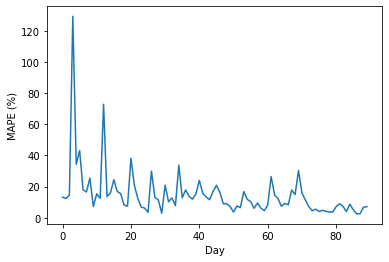
\includegraphics[scale=0.75]{imgs/graphs/full/days_full.png}
    \caption{The recorded Mean Absolute Percentage Error (MAPE) for each day in the test dataset for the full model. 
    \label{fig:days_full}}
\end{figure}




\subsection{Low variance days}
In the test dataset there are a number of clear days, where the sun was mostly or entirely unobstructed. The model predicted most of these days with very low error, in the range 2-5\%. The 90\% confidence interval stayed within $\pm100 W/m^2$ for the whole day and the true prediction was almost spot-on, as can be seen in Fig.~\ref{fig:full_low_best}.
\begin{figure}[ht!]
    \centering
    \subfloat[]{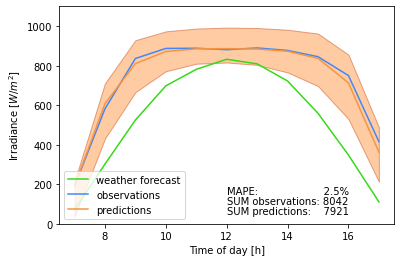
\includegraphics[scale=0.5]{imgs/graphs/full/low/best_3.png}}\qquad
    \subfloat[]{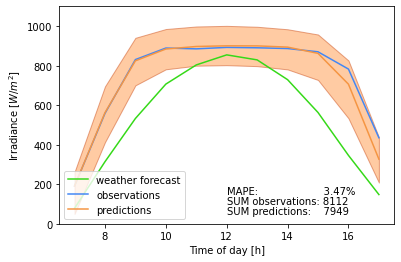
\includegraphics[scale=0.5]{imgs/graphs/full/low/best_2.png}}\qquad
    \caption{Examples of clear days where the model preformed very well.
    \label{fig:full_low_best}}
\end{figure}


The model did not manage near-perfect predictions on all of these clear days, and made a few under-predictions, as can be seen in Fig.~\ref{fig:full_low_worst}.
These predictions were still even and within the 90\% confidence interval, which was slightly larger than for the other clear day predictions. These predictions had a higher MAPE of 10-13\%.
\begin{figure}[ht!]
    \centering
    \subfloat[]{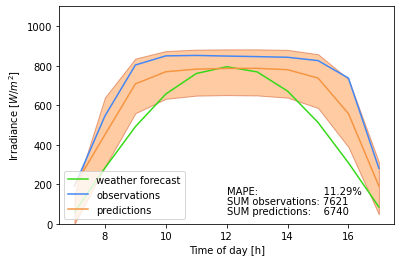
\includegraphics[scale=0.5]{imgs/graphs/full/low/worst_1.png}}\qquad
    \subfloat[]{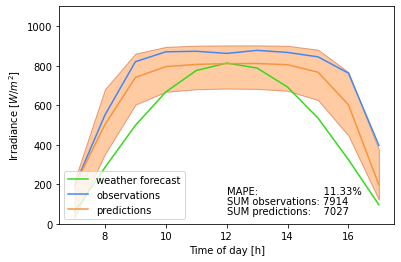
\includegraphics[scale=0.5]{imgs/graphs/full/low/worst_2.png}}\qquad
    \caption{Examples of clear days where the model did not perform well.
    \label{fig:full_low_worst}}
\end{figure}


\subsection{Medium variance days}
On days with some variance in the irradiance measured, the model was generally able to predict the irradiance with relatively good accuracy.
The model has a tendency to give a smoother prediction than the measured value, averaging through the peaks and valleys of the measured values and most of the time the observed value was within the 90\% confidence interval. 

Fig.~\ref{fig:full_med_best} shows examples of good predictions with high confidence, though the confidence is generally lower the farther the irradiance is from the value of a clear day.
\begin{figure}[ht!]
    \centering
    \subfloat[]{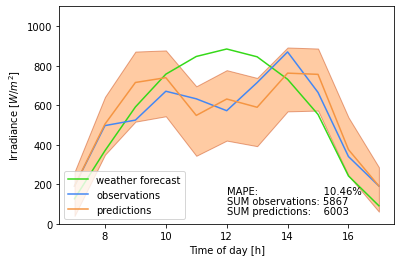
\includegraphics[scale=0.5]{imgs/graphs/full/medium/med_g_1.png}}\qquad
    \subfloat[]{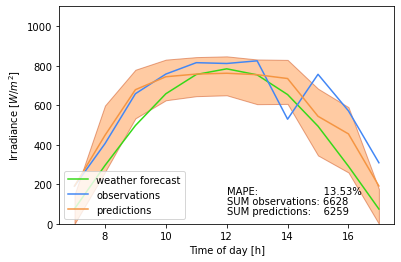
\includegraphics[scale=0.5]{imgs/graphs/full/medium/med_g_2.png}}\qquad
    \subfloat[]{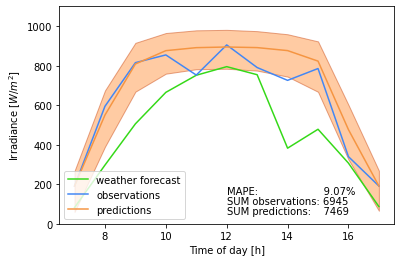
\includegraphics[scale=0.5]{imgs/graphs/full/medium/med_g_3.png}}\qquad
    \subfloat[]{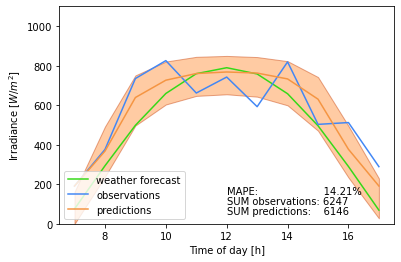
\includegraphics[scale=0.5]{imgs/graphs/full/medium/med_g_4.png}}\qquad
    \caption{Examples of days with some drops in irradiance, where the model performed very well.
    \label{fig:full_med_best}}
\end{figure}

In Fig.~\ref{fig:full_med_med} we can see examples of days where the model achieves higher error, MAPE in the range 19-35\%, but with generally larger 90\% confidence intervals so the model still keeps the measured values close to or within them.
\begin{figure}[ht!]
    \centering
    \subfloat[]{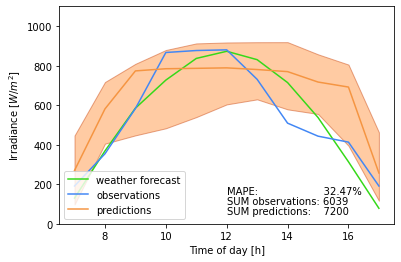
\includegraphics[scale=0.5]{imgs/graphs/full/medium/med_m_1.png}}\qquad
    \subfloat[]{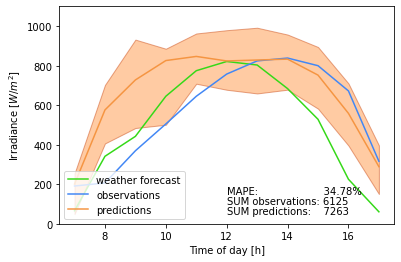
\includegraphics[scale=0.5]{imgs/graphs/full/medium/med_m_2.png}}\qquad
    \subfloat[]{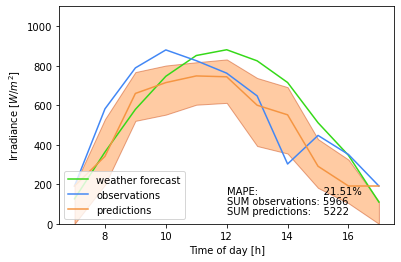
\includegraphics[scale=0.5]{imgs/graphs/full/medium/med_m_3.png}}\qquad
    \subfloat[]{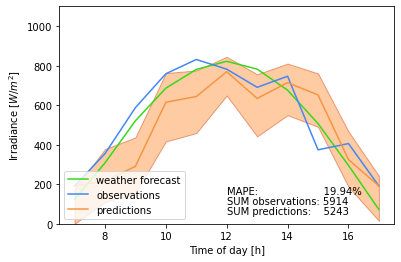
\includegraphics[scale=0.5]{imgs/graphs/full/medium/med_m_4.png}}\qquad
    \subfloat[]{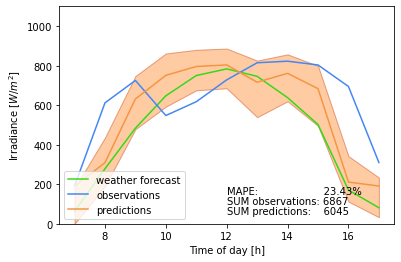
\includegraphics[scale=0.5]{imgs/graphs/full/medium/med_m_5.png}}\qquad
    \caption{Examples of days with some drops in irradiance, where the model performed somewhat well.
    \label{fig:full_med_med}}
\end{figure}

For a few medium variance days, the model did not track well. Figs.~\ref{fig:full_med_bad_a} and \ref{fig:full_med_bad_d} show where the model predicted a constant lower irradiance when half the day had high irradiance and the other half low. Figs.~\ref{fig:full_med_bad_b} and \ref{fig:full_med_bad_c} show the model predicting a mostly or fully  sunny day when it wasn't. In all of these cases, the observed irradiance was far outside the 90\% confidence interval.
\begin{figure}[ht!]
    \centering
    \subfloat[]{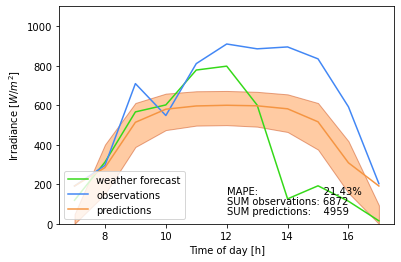
\includegraphics[scale=0.5]{imgs/graphs/full/medium/med_b_1.png}\label{fig:full_med_bad_a}}\qquad
    \subfloat[]{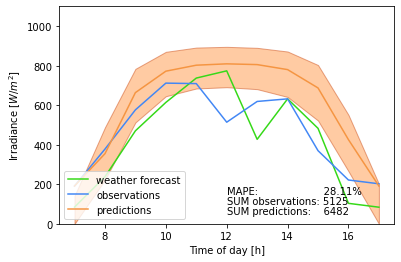
\includegraphics[scale=0.5]{imgs/graphs/full/medium/med_b_2.png}\label{fig:full_med_bad_b}}\qquad
    \subfloat[]{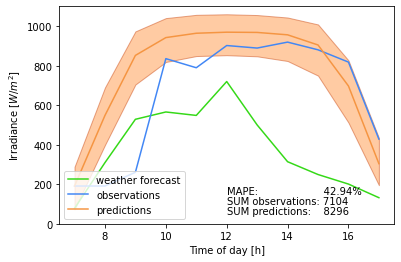
\includegraphics[scale=0.5]{imgs/graphs/full/medium/med_b_3.png}\label{fig:full_med_bad_c}}\qquad
    \subfloat[]{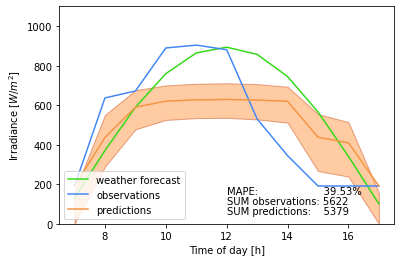
\includegraphics[scale=0.5]{imgs/graphs/full/medium/med_b_4.png}\label{fig:full_med_bad_d}}\qquad
    \caption{Examples of days with some drops in irradiance, where the model performed badly.
    \label{fig:full_med_bad}}
\end{figure}

\clearpage
\subsection{High variance days}
A few days in the dataset had very low irradiance for part of, or the whole day or large fluctuations in irradiance. These situations were most difficult for the model to predict. Figs.~\ref{fig:full_high_a}, \ref{fig:full_high_b} and \ref{fig:full_high_c} show the model somewhat following the observations, but with a high MAPE of 38-80\% because of offsets in time and/or magnitude. The observed value was often outside the 90\% confidence interval of the predictions. For Figs.~\ref{fig:full_high_a}, \ref{fig:full_high_b} the sum of predicted values is close to the sum of observed values, indicating relatively high accuracy for the days taken as a whole. Fig.\ref{fig:full_high_d} shows an outlier with an extremely high MAPE of 139\%, where the model predicts an almost clear day, with high confidence, on a day that receives very little irradiance.
\begin{figure}[ht!]
    \centering
    \subfloat[]{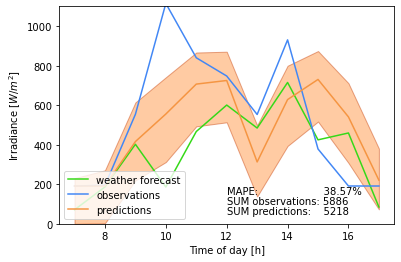
\includegraphics[scale=0.5]{imgs/graphs/full/high/high_1.png}\label{fig:full_high_a}}\qquad
    \subfloat[]{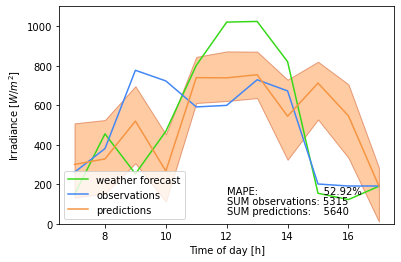
\includegraphics[scale=0.5]{imgs/graphs/full/high/high_2.png}\label{fig:full_high_b}}\qquad
    \subfloat[]{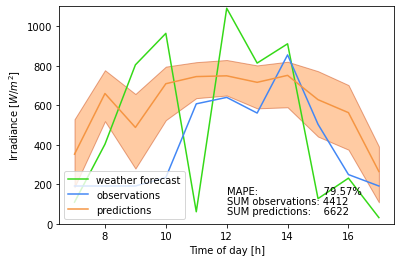
\includegraphics[scale=0.5]{imgs/graphs/full/high/high_3.png}\label{fig:full_high_c}}\qquad
    \subfloat[]{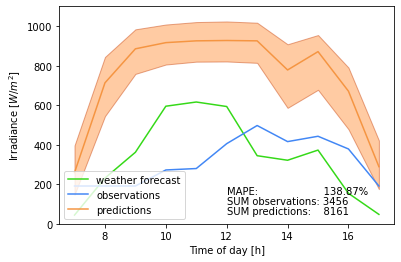
\includegraphics[scale=0.5]{imgs/graphs/full/high/high_4.png}\label{fig:full_high_d}}\qquad
    \caption{Examples of days with large drops in irradiance or low irradiance throughout.
    \label{fig:full_high}}
\end{figure}




\clearpage
\section{Less forecast data}
The limited model, utilizing irradiance data only from the one forecast region, and not surrounding regions, achieved an average MAPE of 15.98\% on the test dataset. The maximum daily average MAPE was 122.87\% and the minimum was 3.47\%. 
\begin{figure}[ht!]
    \centering
    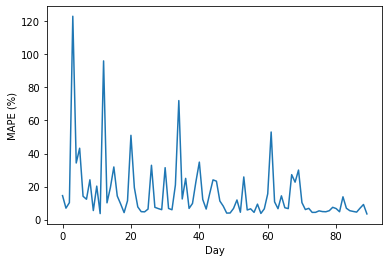
\includegraphics[scale=0.75]{imgs/graphs/less/days_single.png}
    \caption{The recorded Mean Absolute Percentage Error for each day in the test dataset of the limited model. 
    \label{fig:days_less}}
\end{figure}


\subsection{Low variance days}
The model predicts most clear days with relatively high accuracy, but even on the best days it deviates from the quite a bit from the observed values, as shown in Fig.~\ref{fig:less_low_a}. The model sometimes under-predicts on clear days. In Fig.~\ref{fig:less_low_b} we can see an example of a day where, even though the 90\% confidence area is large, the observed irradiance is outside it.
\begin{figure}[ht!]
    \centering
    \subfloat[]{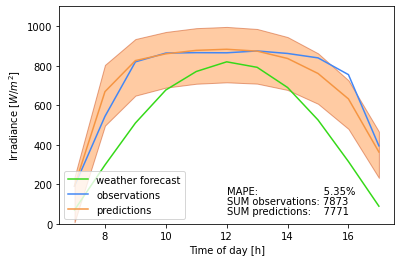
\includegraphics[scale=0.5]{imgs/graphs/less/low/low_g_1.png}\label{fig:less_low_a}}\qquad
    \subfloat[]{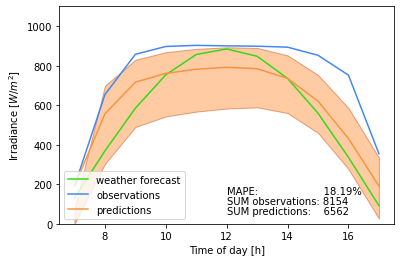
\includegraphics[scale=0.5]{imgs/graphs/less/low/low_b_1.png}\label{fig:less_low_b}}\qquad
    \caption{Examples of model performance on clear days.
    \label{fig:less_low}}
\end{figure}


\subsection{Medium variance days}
The model shows less accuracy when the irradiance is not steady. Predictions for most days have the smooth profile of an optimal day, but are scaled to fit closer to the lower total irradiance for the day. The model is inconsistent in how well it tracks the observed irradiance and the confidence it does that with. Sometimes, as shown in Fig.~\ref{fig:less_med_a} the model tracks relatively well, with the observations mostly within the rather tight 90\% confidence interval of roughly $+50/-150 W/m^2$. In Fig.~\ref{fig:less_med_b} we see an example where the model was wrong with very high confidence for the first half of the day. Fig.~\ref{fig:less_med_c} shows the opposite, the model predicts low irradiance for the whole day with a very large 90\% confidence interval of roughly $\pm200 W/m^2$.
\begin{figure}[ht!]
    \centering
    \subfloat[]{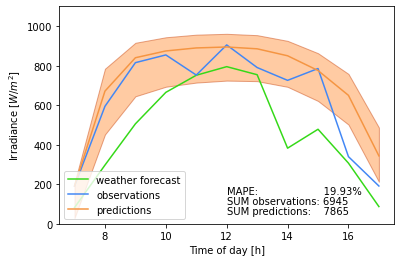
\includegraphics[scale=0.5]{imgs/graphs/less/medium/med_g_1.png}\label{fig:less_med_a}}\qquad
    \subfloat[]{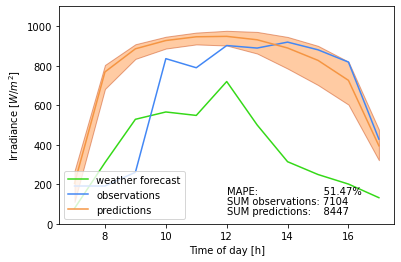
\includegraphics[scale=0.5]{imgs/graphs/less/medium/med_m_2.png}\label{fig:less_med_b}}\qquad
    \subfloat[]{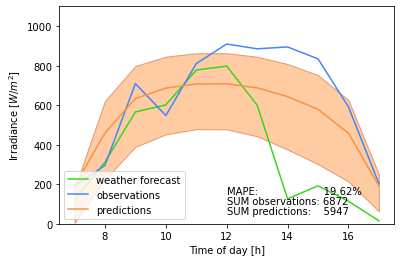
\includegraphics[scale=0.5]{imgs/graphs/less/medium/med_m_1.png}\label{fig:less_med_c}}\qquad
    \caption{Examples of days with some drops in irradiance.
    \label{fig:less_med}}
\end{figure}

\clearpage
\subsection{High variance days}
For the few days in the dataset that had very low irradiance for part of, or the whole day or large fluctuations in irradiance, the model showed high error, MAPE in the range 53-123\% with varying confidence. Figs.~\ref{fig:less_high_a} and \ref{fig:less_high_b} show large over-predictions with high confidence, and Figs.~\ref{fig:less_high_c} and \ref{fig:less_high_d} show days where the 90\% confidence interval covered the top 60\% of the graph, yet it did not cover the observations.
\begin{figure}[ht!]
    \centering
    \subfloat[]{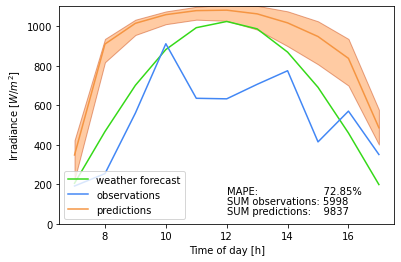
\includegraphics[scale=0.5]{imgs/graphs/less/high/high_1.png}\label{fig:less_high_a}}\qquad
    \subfloat[]{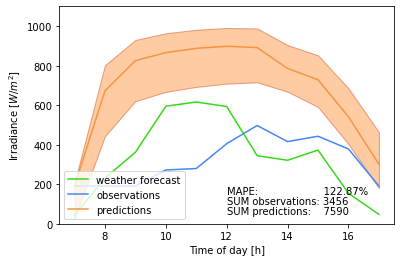
\includegraphics[scale=0.5]{imgs/graphs/less/high/high_2.png}\label{fig:less_high_b}}\qquad
    \subfloat[]{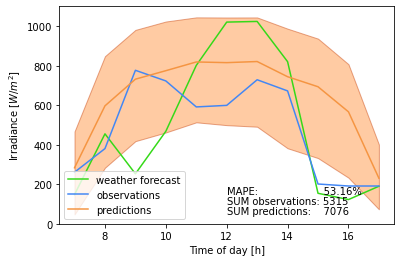
\includegraphics[scale=0.5]{imgs/graphs/less/high/high_3.png}\label{fig:less_high_c}}\qquad
    \subfloat[]{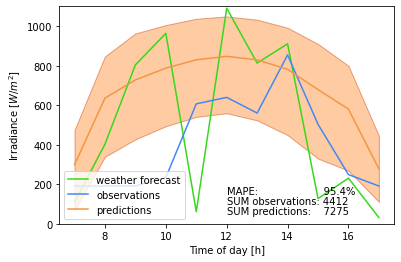
\includegraphics[scale=0.5]{imgs/graphs/less/high/high_4.png}\label{fig:less_high_d}}\qquad
    \caption{Examples of days with large drops in irradiance or low irradiance throughout.
    \label{fig:less_high}}
\end{figure}